%%% Поля и разметка страницы %%%
\documentclass[a4paper,12pt]{article}


\textwidth=175mm
\textheight=260mm
\oddsidemargin=-.4mm
\headsep=5mm

\topmargin=-1in
\unitlength=1mm

\usepackage{lscape}		% Для включения альбомных страниц

%%% Кодировки и шрифты %%%
\usepackage{cmap}						% Улучшенный поиск русских слов в полученном pdf-файле
\usepackage[T2A]{fontenc}				% Поддержка русских букв
\usepackage[utf8]{inputenc}				% Кодировка utf8
\usepackage[english, russian]{babel}	% Языки: русский, английский
% \usepackage{pscyr}						% Красивые русские шрифты

%%% Математические пакеты %%%
\usepackage{amsthm,amsfonts,amsmath,amssymb,amscd,mathrsfs} % Математические дополнения от AMS

%%% Оформление абзацев %%%
%\usepackage{indentfirst} % Красная строка

%%% Цвета %%%
\usepackage[usenames]{color}
\usepackage{color}
\usepackage{colortbl}

%%% Таблицы %%%
\usepackage{longtable}					% Длинные таблицы
\usepackage{multirow,makecell,array}	% Улучшенное форматирование таблиц

%%% Общее форматирование
\usepackage[singlelinecheck=off,center]{caption}	% Многострочные подписи
\usepackage{soul}									% Поддержка переносоустойчивых подчёркиваний и зачёркиваний

%%% Библиография %%%
\usepackage{cite} % Красивые ссылки на литературу

%%% Гиперссылки %%%
\usepackage[plainpages=false,pdfpagelabels=false]{hyperref}
\definecolor{linkcolor}{rgb}{0.9,0,0}
\definecolor{citecolor}{rgb}{0,0.6,0}
\definecolor{urlcolor}{rgb}{0,0,1}
\hypersetup{
colorlinks, linkcolor={linkcolor},
citecolor={citecolor}, urlcolor={urlcolor}
}

%%% Изображения %%%
\usepackage{graphicx}		% Подключаем пакет работы с графикой
\graphicspath{{images/}}	% Пути к изображениям

%%% Выравнивание и переносы %%%
\sloppy					% Избавляемся от переполнений
\clubpenalty=10000		% Запрещаем разрыв страницы после первой строки абзаца
\widowpenalty=10000		% Запрещаем разрыв страницы после последней строки абзаца


\usepackage{tikz}

\graphicspath{ {./} }

\DeclareMathOperator*{\mycup}{\cup}
\DeclareMathOperator*{\mycap}{\cap}

%%%%%%%%%%%%%%%%%%%%%%%%%%%%%%%%%%%%%%%%%%%%%%%%%%%%%%%%%%%%%%%%%%%%%%%%%%%%%%%%%%%
\begin{document}
\begin{center}
\Huge{Домашнее задание по курсу $"$Математическая логика - 2$"$}
\end{center}

\section{Язык и аксиоматика теории множеств}
\subsection*{$\S$ 1.3}
\paragraph*{Условие}
Доказать, что $\varnothing \not= 	\{ \varnothing \}.$
\paragraph*{Доказательство}
По определению\\
$ x = y \rightleftharpoons \forall t ( t \in x \Leftrightarrow t \in y ).$\\
Пусть $\varnothing = 	\{ \varnothing \} $,
$ \Rightarrow \forall t ( t \in \{ \varnothing \} \Leftrightarrow t \in \varnothing )$
Противоречие для t = $ \varnothing $

\subsection*{$\S$ 1.4}
\paragraph*{Условие}
Доказать, что $\{\{1, 2\}, \{2,3\}\} \not= 	\{ 1,2,3 \}. $
\paragraph*{Доказательство}
По определению\\
$ x = y \rightleftharpoons \forall t ( t \in x \Leftrightarrow t \in y ).$\\
Пусть $\{\{1, 2\}, \{2,3\}\} = 	\{ 1,2,3 \} $,
$ \Rightarrow \forall t ( t \in \{ 1,2,3 \} \Leftrightarrow t \in \{\{1, 2\}, \{2,3\}\} )$
Противоречие для t = $ 1 $

\subsection*{$\S$ 1.6}
\paragraph*{Условие}
Доказать, что $\exists$ лишь одно множество, не имеющее элементов.
\paragraph*{Доказательство}
Пусть $\exists$ два множества X и $X_0$, не имеющих элементов и такие, что $X \not= X_0$\\
$ \Rightarrow \exists t ( t \in X \Rightarrow  t \not\in X_0 )$ или $\exists t ( t \in X_0 \Rightarrow  t \not\in X )$ \\
Противоречие так как $\nexists t \in X$ и $\nexists t \in X_0$.

\subsection*{$\S$ 1.8}
\paragraph*{Условие}
Доказать, что множество всех корней многочлена $\alpha (x)=\beta (x) \gamma (x)$ есть объединение множеств корней $\beta (x)$ и $\gamma(x)$.
\paragraph*{Доказательство}
Чтобы докаказать, что множество корней = объединения множеств, надо доказать, что любой корень является либо корнем $\beta (x)$ либо $\gamma(x)$ и что других корней не существует.\\
1) Пусть существует корень $x_0$, который не является корнем ни $\beta (x)$, ни корнем $\gamma(x)$ \\
$\Rightarrow \alpha (x_0) = 0, \beta (x_0) \not= 0,  \gamma (x_0) \not= 0$. Противоречие
2) Пусть $x_0$ корень $\beta (x)$ или  $\gamma(x)$ , тогда  $\beta (x_0) = 0$ или $\gamma(x_0) = 0$ $\Rightarrow \alpha(x_0) = 0$

\subsection*{$\S$ 1.9}
\paragraph*{Условие}
Доказать, что персечение множеств действительных корней многочленов  $\alpha (x) и \beta (x)$ с действительными коэффицентами  совпадает с множеством всех действительных корней $\gamma(x) =\alpha^2 (x) + \beta^2 (x)  $.
\paragraph*{Доказательство}
Чтобы докаказать, что множество корней = персечение множеств, надо доказать, что любой корень из пересейчения является корнем и что других корней не существует.\\
1)Если $x_0$ корень $\alpha (x) и \beta (x)$ $\Rightarrow$ $\gamma(x_0) = 0$
2)Пусть существует корень  $\gamma(x) x_0$, который не является корнем ни $\alpha (x)$, ни корнем $\beta(x)$ \\
Тогда $\gamma(x_0) = 0$ $\Rightarrow \alpha^2 (x_0) + \beta^2 (x_0) = 0 \Rightarrow  \alpha(x_0) =  0 \& \beta (x_0) = 0$

\subsection*{$\S$ 1.11 (а, г, ж)}
\paragraph*{Условие}
Доказать следующие тождества\\
a)$ A \cup A = A \cap A = A $
\paragraph*{Доказательство}
Распишем по определению\\
$\{ Z \mid (Z \in A \vee Z \in A)\} = \{ Z \in A \cup A \mid Z \in A \wedge Z \in A \} = A $\\
Упростим\\
$\{ Z \mid (Z \in A )\} = \{ Z \in A \cup A \mid Z \in A \} = A $ $\Leftrightarrow$ $ A = \{ Z \in A  \mid Z \in A \} = A $  $\Leftrightarrow$ $A=A=A$
\paragraph*{Условие}
г)$ A \cap ( B \cap C ) = ( A \cap B ) \cap C$
\paragraph*{Доказательство} \mbox{}\\
\def\firstcircle{(0,0) circle (1.5cm)}
\def\secondcircle{(45:2cm) circle (1.5cm)}
\def\thirdcircle{(0:2cm) circle (1.5cm)}
\begin{tikzpicture}
	\begin{scope}[shift={(0cm,6cm)}, fill opacity=0.8]
		\begin{scope}% first circle without the second
			\clip \secondcircle;
      		\fill[red] \thirdcircle;
        \end{scope}
        \begin{scope}% first circle without the second
			 \clip \firstcircle;
      		\clip \secondcircle;
     		 \fill[green] \thirdcircle;
        \end{scope}
        \draw \firstcircle node {$A$};
        \draw \secondcircle node {$B$};
        \draw \thirdcircle node {$C$};
    \end{scope}

	 \begin{scope}[shift={(6cm,6cm)}, fill opacity=0.8]
	 	\begin{scope}% first circle without the second
			\clip \firstcircle;
      		\fill[red] \secondcircle;
        \end{scope}
	 	\begin{scope}% first circle without the second
			 \clip \firstcircle;
      		\clip \secondcircle;
     		 \fill[green] \thirdcircle;
        \end{scope}
        \draw \firstcircle node {$A$};
        \draw \secondcircle node  {$B$};
        \draw \thirdcircle node {$C$};
    \end{scope}
\end{tikzpicture}

\paragraph*{Условие}
ж)$A \cup ( B \cap C ) = ( A \cup B ) \cap ( A \cup C )$
\paragraph*{Доказательство} \mbox{}\\

\begin{tikzpicture}
	\begin{scope}[shift={(0cm,6cm)}, fill opacity=0.5]
		\begin{scope}% first circle without the second
			\clip \secondcircle;
      		\fill[red] \thirdcircle;
        \end{scope}
        \begin{scope}% first circle without the second
     		 \fill[green] \firstcircle;
     		 \clip \secondcircle;
      		\fill[green] \thirdcircle;
        \end{scope}

        \draw \firstcircle node {$A$};
        \draw \secondcircle node {$B$};
        \draw \thirdcircle node {$C$};
    \end{scope}

	 \begin{scope}[shift={(6cm,6cm)}, fill opacity=0.5]
	 	\begin{scope}% first circle without the second
	 		\fill[red] \firstcircle;
	 		\fill[red] \secondcircle;
        \end{scope}
        \begin{scope}% first circle without the second
			\fill[yellow] \firstcircle;
      		\fill[yellow] \thirdcircle;
        \end{scope}
	 	\begin{scope}% first circle without the second
        \end{scope}
        \draw \firstcircle node {$A$};
        \draw \secondcircle node  {$B$};
        \draw \thirdcircle node {$C$};
    \end{scope}
\end{tikzpicture}

\subsection*{$\S$ 1.12(в, д, ж, п, т)}
\begin{center}
  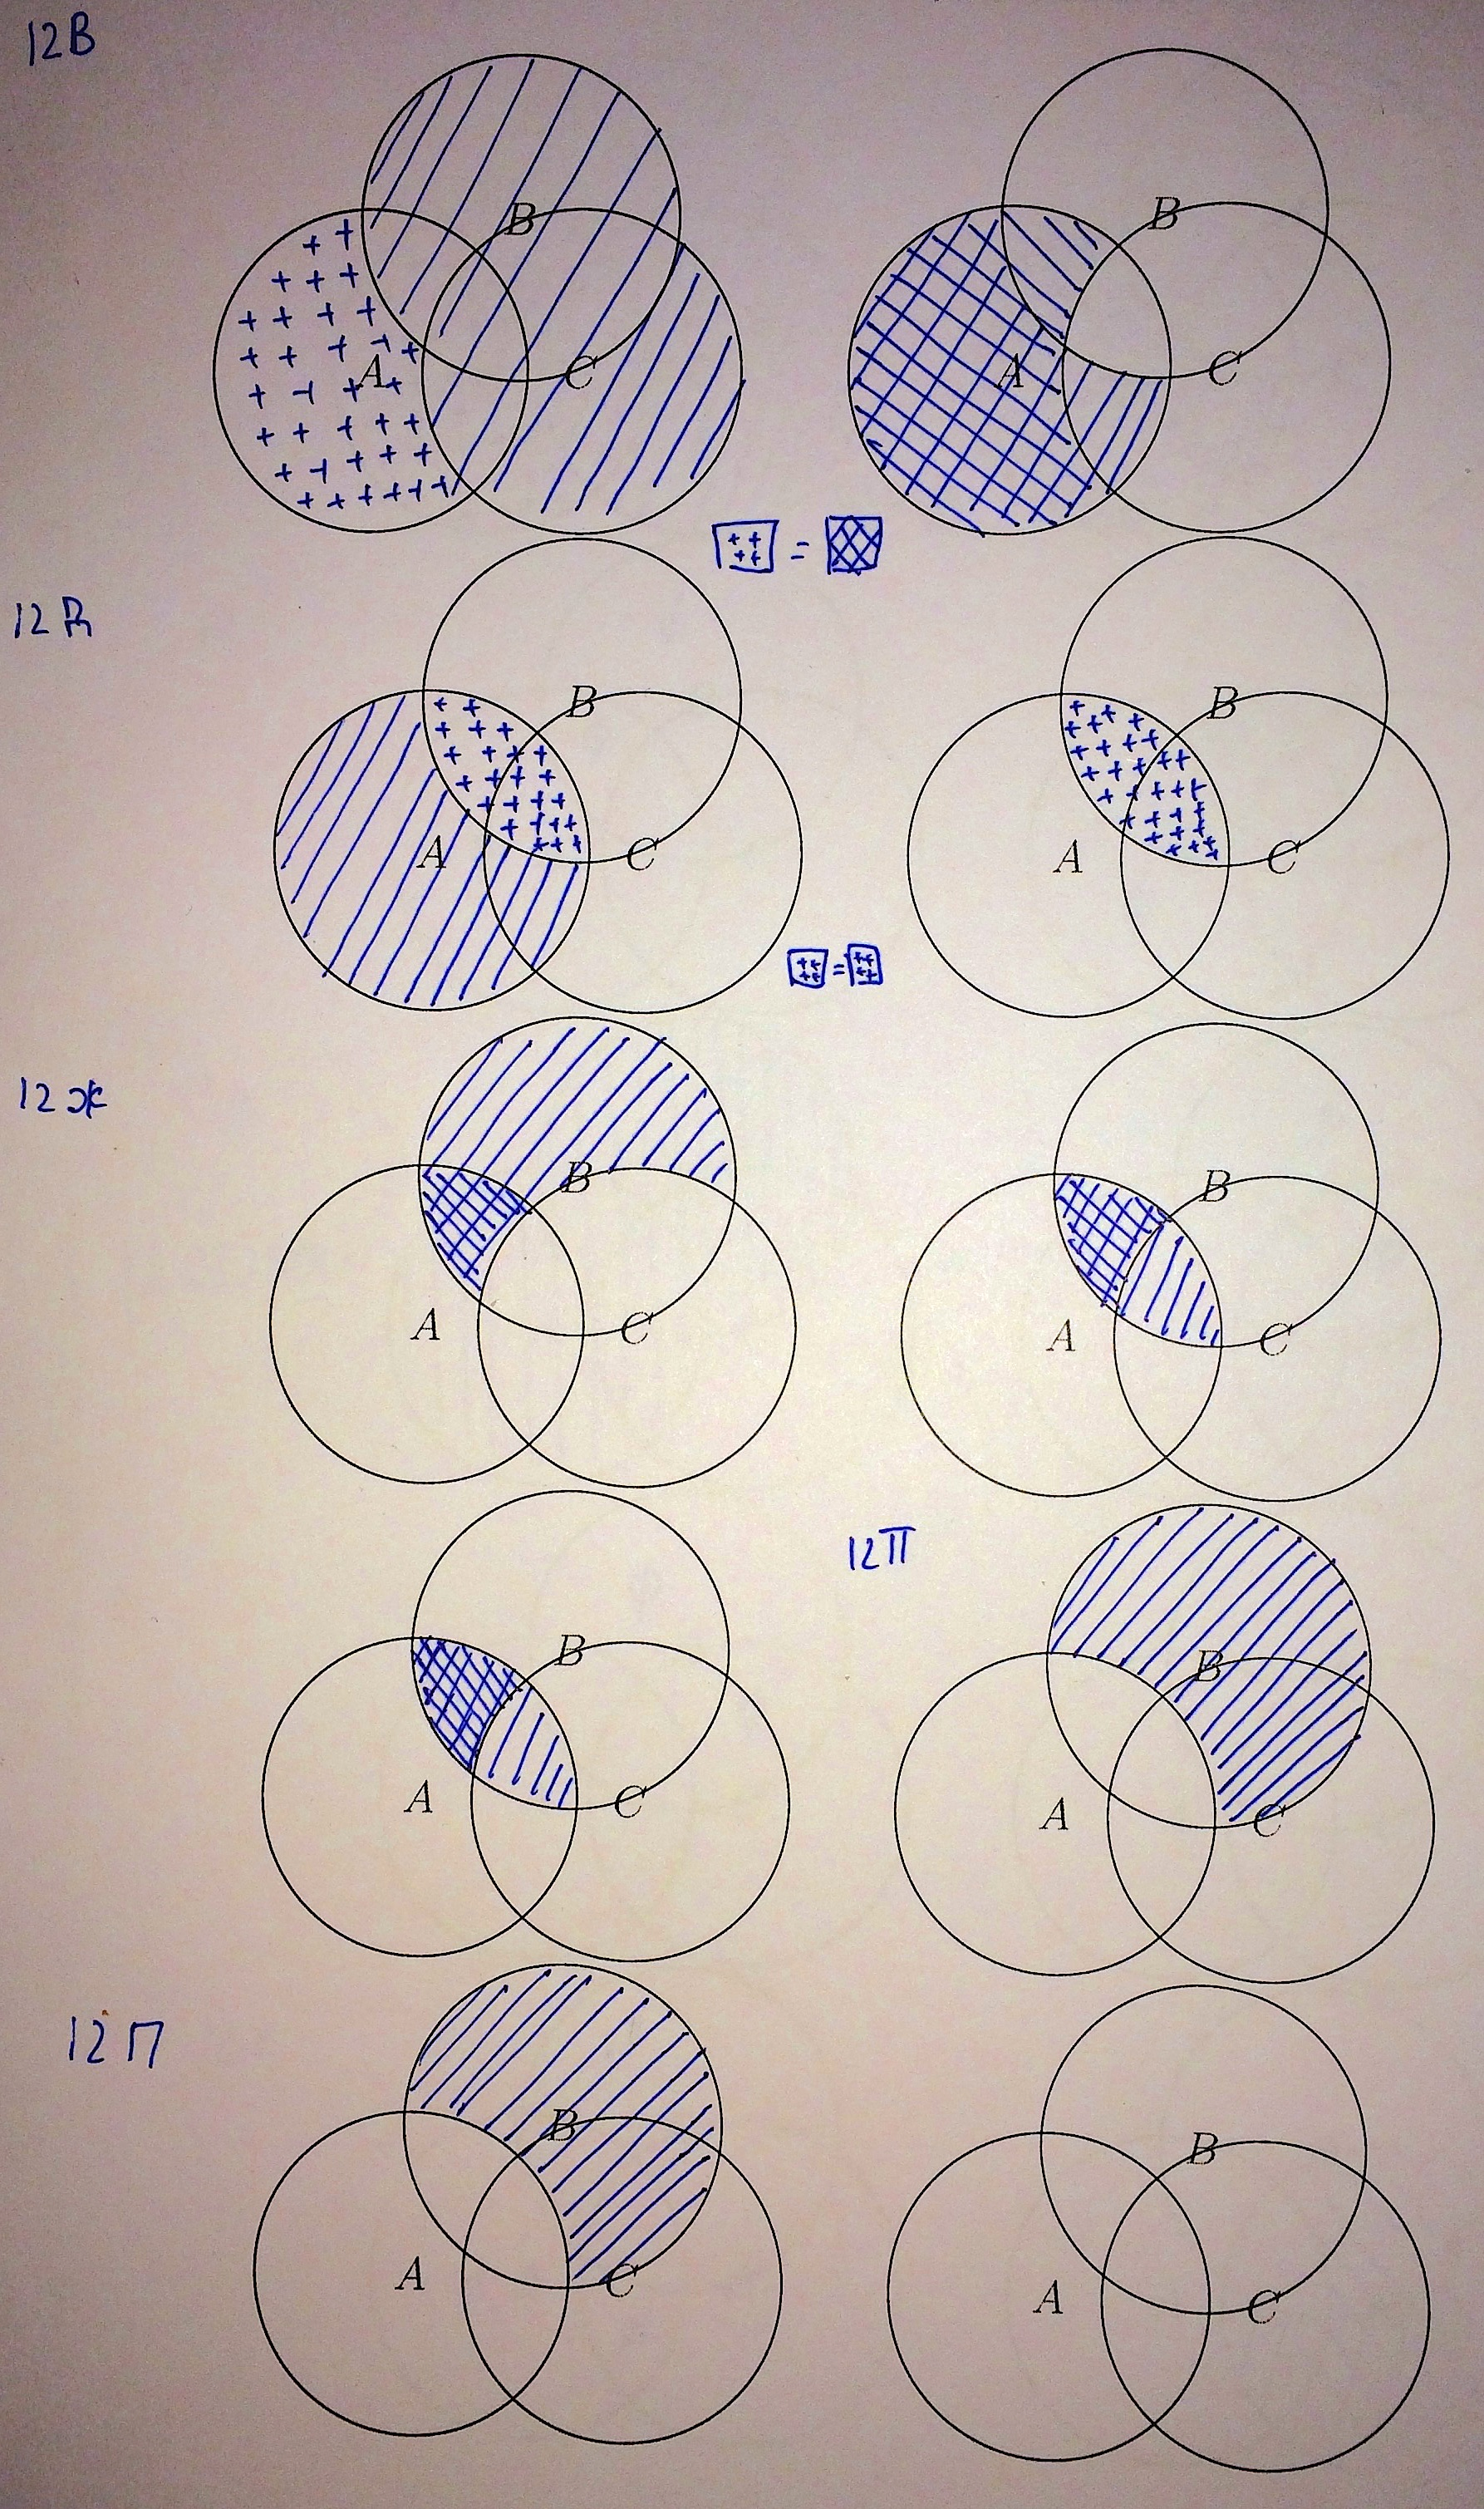
\includegraphics[scale=0.15]{img/1.jpg}
\end{center}
\subsection*{$\S$ 1.13(а, д, к)}
\begin{center}
  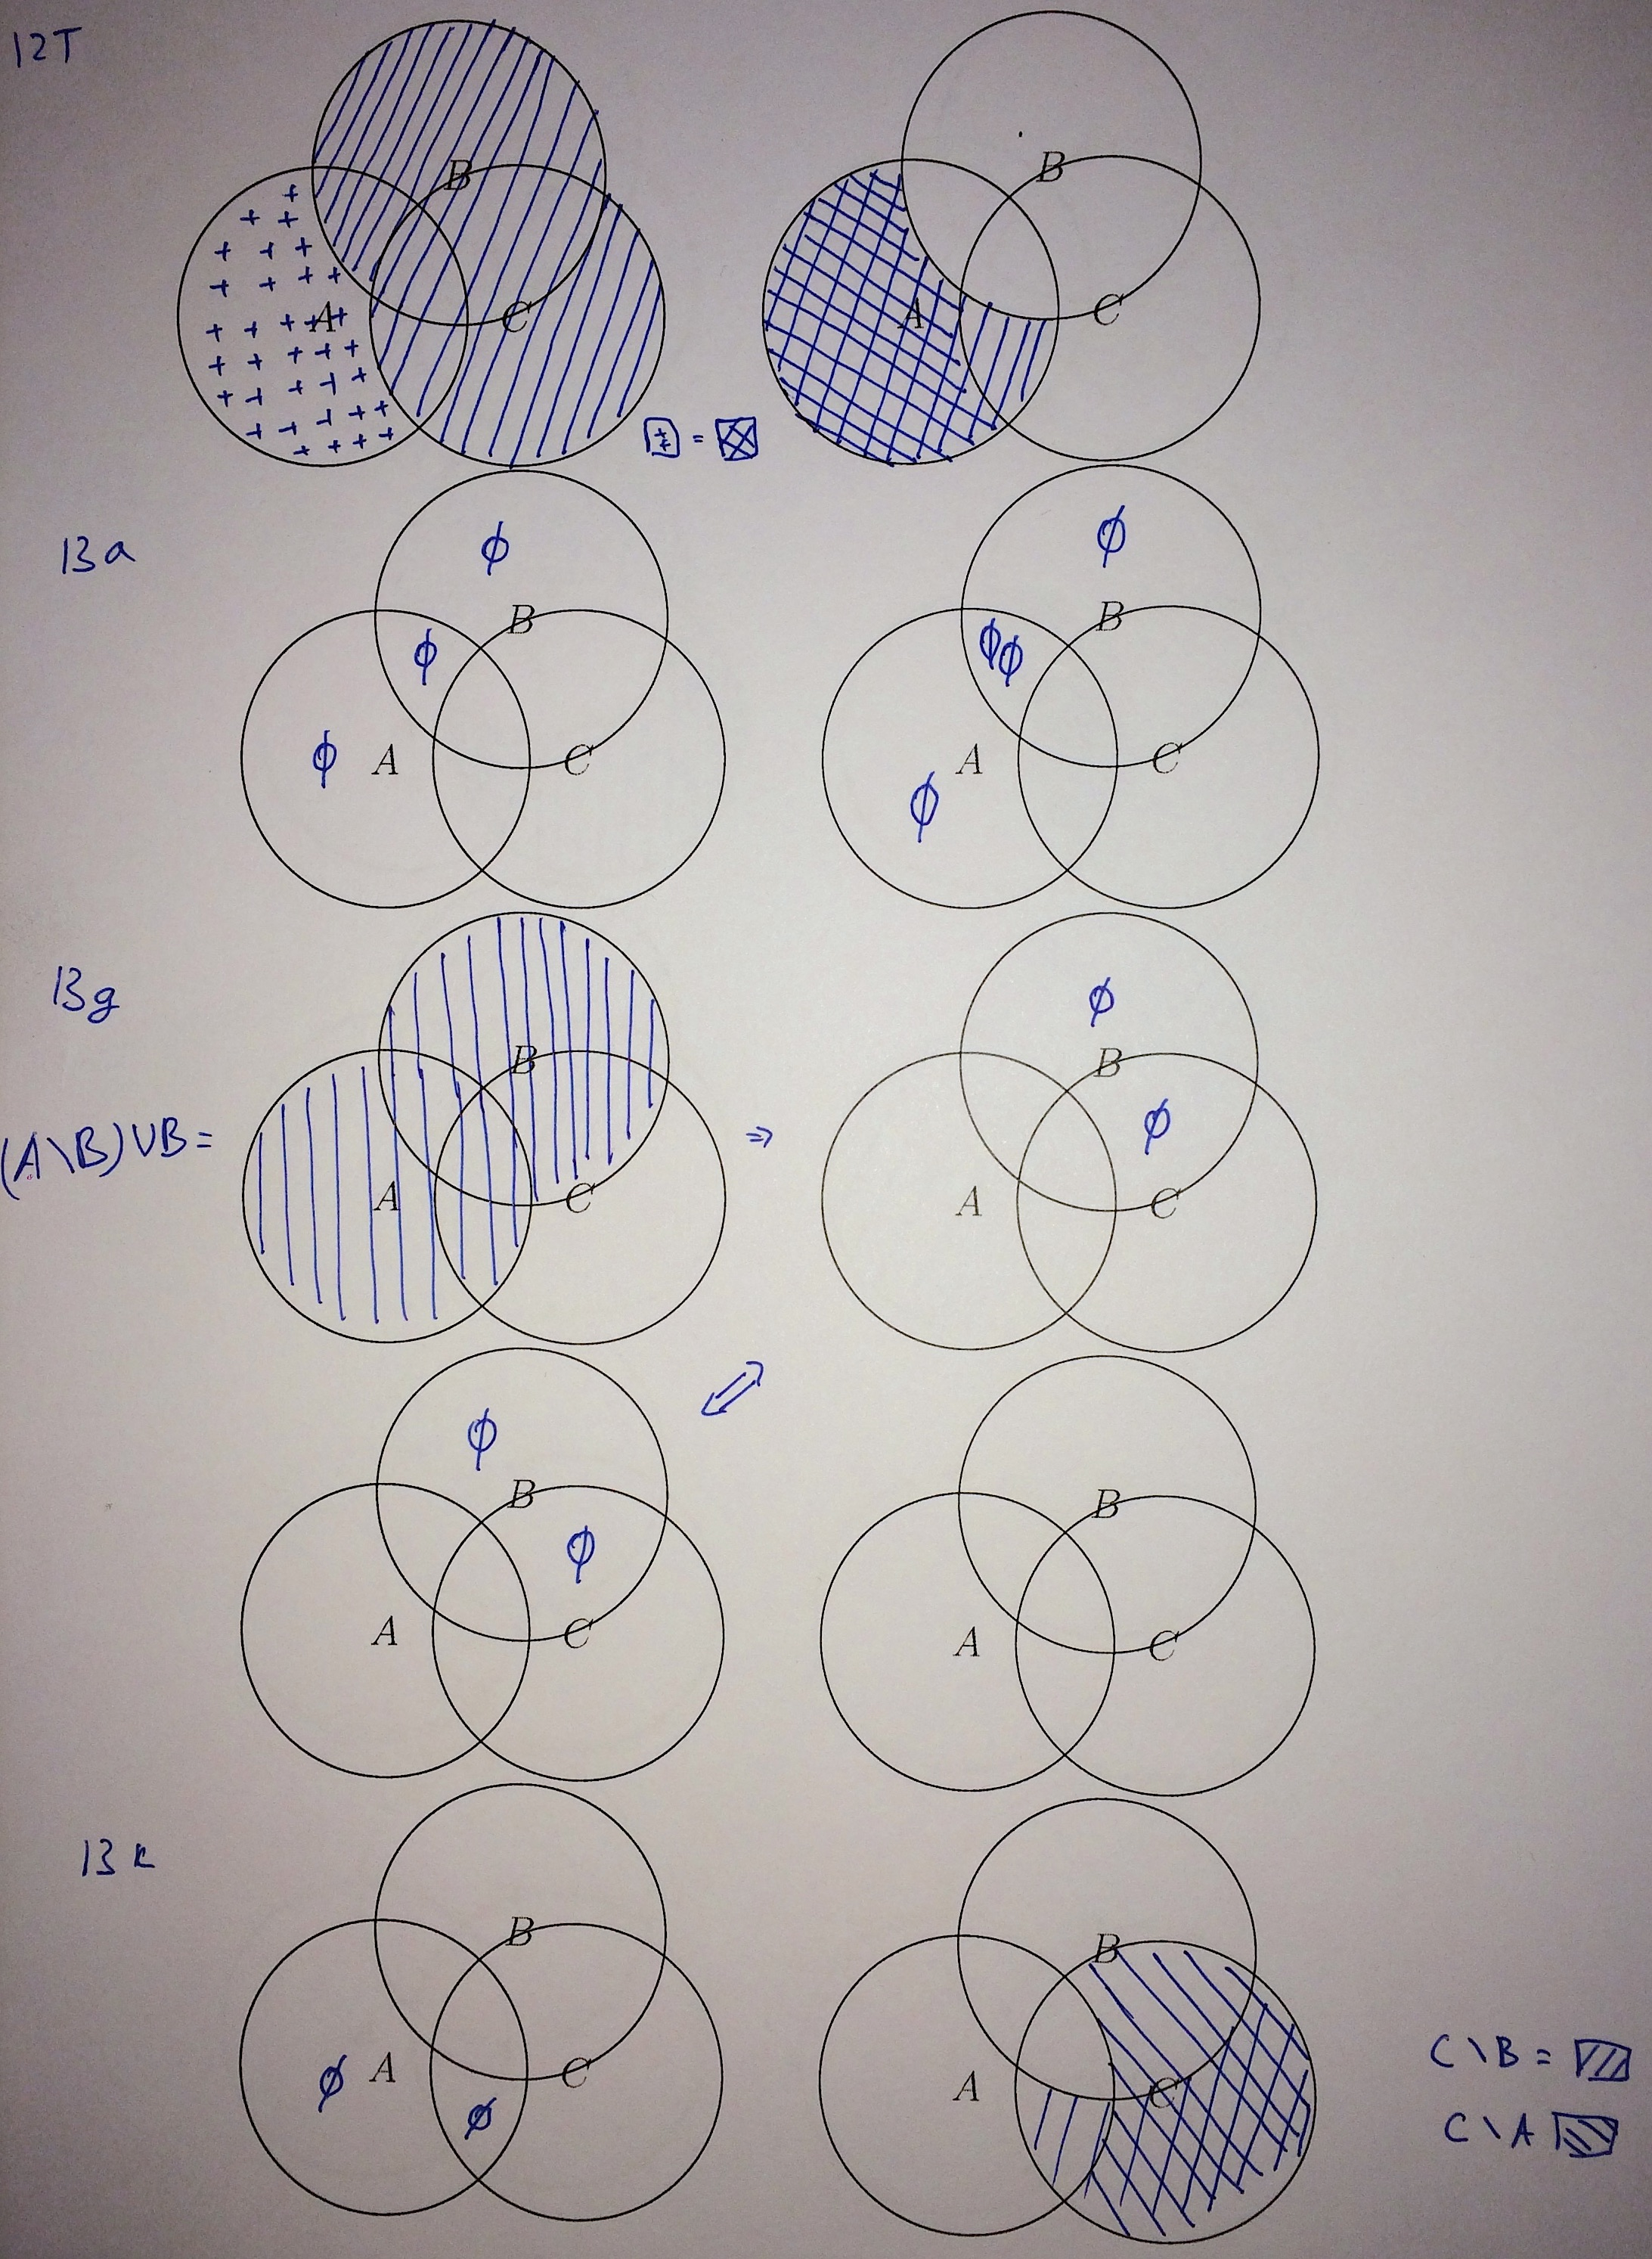
\includegraphics[scale=0.15]{img/2.jpg}
\end{center}
\subsection*{$\S$ 1.14(в, к)}
\begin{center}
  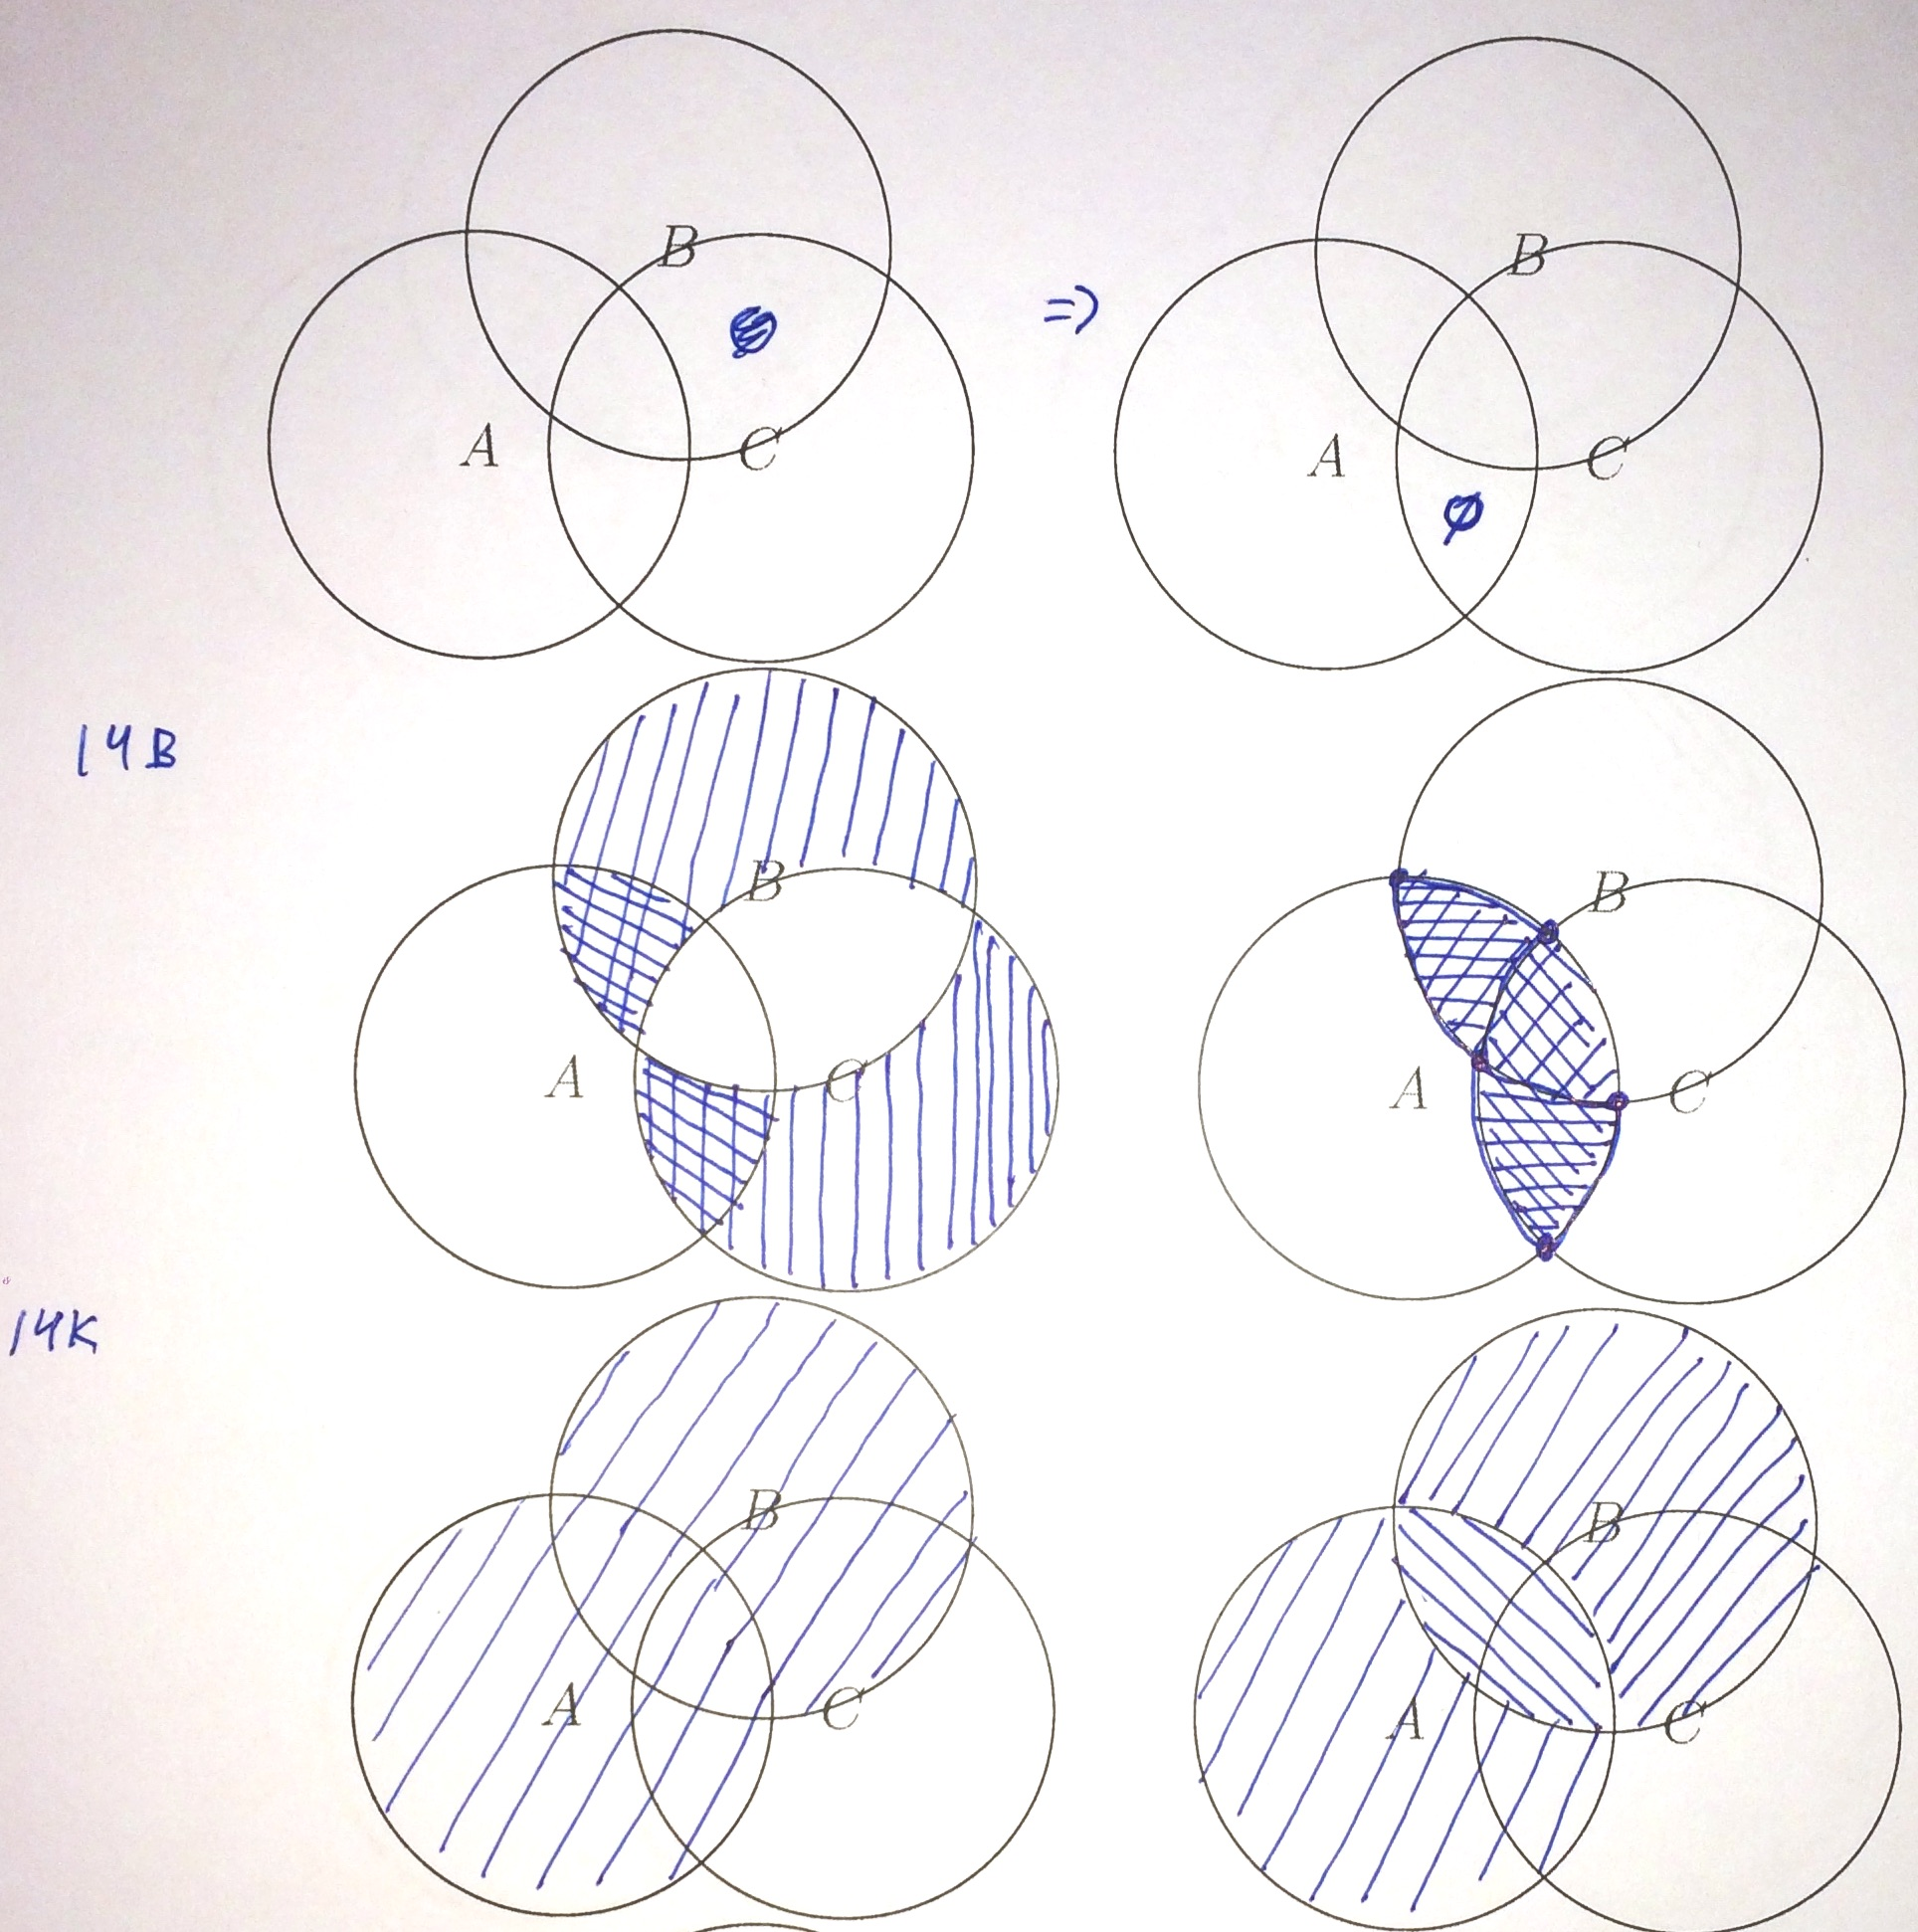
\includegraphics[scale=0.15]{img/3.jpg}
\end{center}
\subsection*{$\S$ 1.15}
\paragraph*{Условие}
Доказать, что\\
a) $(A_1 \cup ... \cup A_n) \bigtriangleup (B_1 \cup ... \cup B_n) \subseteq (A_1 \bigtriangleup B_1) \cup ... \cup (A_n \bigtriangleup B_n) $
\paragraph*{Доказательство}
Докажем по индукции:\\
\textbf{База индукции}\\
 n=1)  $(A_1) \bigtriangleup (B_1) \subseteq (A_1 \bigtriangleup B_1) $ (очевидно)\\
 n=2)  $(A_1 \cup  A_2) \bigtriangleup (B_1 \cup B_2) \subseteq (A_1 \bigtriangleup B_1) \cup (A_2 \bigtriangleup B_2) $(Доказывалось на уроке)\\
 \textbf{Преположение индукции}\\
 Пусть верно для $\forall n < k$\\
 \textbf{Шаг индукции}\\
 Докажем для k+1\\
 $(A_1 \cup ... \cup A_{k+1}) \bigtriangleup (B_1 \cup ... \cup B_{k+1}) \subseteq (A_1 \bigtriangleup B_1) \cup ... \cup (A_{k+1} \bigtriangleup B_{k+1}) $\\
 пусть $ A_0 = A_1 \cup ... \cup A_k и B_0 = B_1 \cup ... \cup B_k$\\
 $(A_1 \cup ... \cup A_{k+1}) \bigtriangleup (B_1 \cup ... \cup B_{k+1}) \Leftrightarrow (A_0 \cup A_{k+1}) \bigtriangleup (B_0 \cup B_{k+1}) \subseteq $ \\
$ \subseteq (A_0 \bigtriangleup B_0) \cup (A_k \bigtriangleup B_k)$\\
$(A_0 \bigtriangleup B_0) \subseteq  (A_1 \bigtriangleup B_1) \cup ... \cup (A_k \bigtriangleup B_k)$\\
$\Rightarrow (A_1 \cup ... \cup A_{k+1}) \bigtriangleup (B_1 \cup ... \cup B_{k+1}) \subseteq (A_1 \bigtriangleup B_1) \cup ... \cup (A_{k+1} \bigtriangleup B_{k+1}) $

\paragraph*{Условие}
б) $(A_1 \cap ... \cap A_n) \bigtriangleup (B_1 \cap ... \cap B_n) \subseteq (A_1 \bigtriangleup B_1) \cup ... \cup (A_n \bigtriangleup B_n) $
\paragraph*{Доказательство}
Докажем по индукции:\\
\textbf{База индукции}\\
 n=1)  $(A_1) \bigtriangleup (B_1) \subseteq (A_1 \bigtriangleup B_1) $ (очевидно)\\
 n=2)  $(A_1 \cap  A_2) \bigtriangleup (B_1 \cap B_2) \subseteq (A_1 \bigtriangleup B_1) \cup (A_2 \bigtriangleup B_2) $(Доказывалось на уроке)\\
 \textbf{Преположение индукции}\\
 Пусть верно для $\forall n < k$\\
 \textbf{Шаг индукции}\\
 Докажем для k+1\\
 $(A_1 \cap ... \cap A_{k+1}) \bigtriangleup (B_1 \cap ... \cap B_{k+1}) \subseteq (A_1 \bigtriangleup B_1) \cup ... \cup (A_{k+1} \bigtriangleup B_{k+1}) $\\
 пусть $ A_0 = A_1 \cap ... \cap A_k и B_0 = B_1 \cap ... \cap B_k$\\
 $(A_1 \cap ... \cap A_{k+1}) \bigtriangleup (B_1 \cap ... \cap B_{k+1}) \Leftrightarrow (A_0 \cap A_{k+1}) \bigtriangleup (B_0 \cap B_{k+1}) \subseteq $ \\
$ \subseteq (A_0 \bigtriangleup B_0) \cup (A_k \bigtriangleup B_k)$\\
$(A_0 \bigtriangleup B_0) \subseteq  (A_1 \bigtriangleup B_1) \cup ... \cup (A_k \bigtriangleup B_k)$\\
$\Rightarrow (A_1 \cap ... \cap A_{k+1}) \bigtriangleup (B_1 \cap ... \cap B_{k+1}) \subseteq (A_1 \bigtriangleup B_1) \cup ... \cup (A_{k+1} \bigtriangleup B_{k+1}) $\\

\subsection*{$\S$ 1.17}
\paragraph*{Условие}
Определить операции $ \cup,  \cap,  \setminus$, через:\\
a)$\bigtriangleup, \cap$
\paragraph*{Доказательство} \mbox{}\\
$\cap = \cap $\\
$ A \cup B = (A \bigtriangleup B) \bigtriangleup ( A \cap B)$\\
$ A \setminus B =  (A \bigtriangleup B) \cap A$
\paragraph*{Условие}
б)$\bigtriangleup, \cup$
\paragraph*{Доказательство} \mbox{}\\
$\cup = \cup $\\
$ A \cap B = ((A \cup B) \bigtriangleup A) \bigtriangleup B $\\
$ A \setminus B =  (A \cup B) \bigtriangleup B$
\paragraph*{Условие}
и)$\setminus, \bigtriangleup$
\paragraph*{Доказательство} \mbox{}\\
$ A \cup B = (A \setminus B) \bigtriangleup $\\
$ A \cap B = (B \setminus (A \setminus B)) $\\
$ \setminus =  \setminus$

\subsection*{$\S$ 1.18}
\paragraph*{Условие}
Доказать, что нельзя определить:\\
a) $\setminus$ через $\cap$ и $\cup $\\
б) $\cup$ через $\cap$ и $\setminus $
\paragraph*{Решение} \mbox{}\\
a)Пусть можно, тогда подставим в это определение непустое множества A и A - их симметрическая разница равна $\varnothing$, но объединение пересечение могут дать только само A\\
б)Возьмем 2 конечных непересекащихся множества после выполенеия операций $\cap$ и $\setminus $ размер множества не больше, чем максимальное из множество. Но объединение двух множеств дает множество размером суммы размеров. Значит размеры будут разные. $\rightarrow$ нельзя определить.

\subsection*{$\S$ 1.20}
\paragraph*{Условие}
Найти все подмножества множеств:$\varnothing, \{ \varnothing \}, \{ x \}, \{1, 2\}. $
\paragraph*{Ответ} \mbox{}\\
$\varnothing $ - нет\\
$\{ \varnothing \} - \varnothing$\\
$\{ x \} - \varnothing, \{x\}$\\
$\{1, 2\} - \varnothing, \{1\}, \{2\}, \{1, 2\}$

\subsection*{$\S$ 2.1}
\paragraph*{Условие}
Доказать, что существуют A, B и C такие, что:\\
а) $A \times B \neq B \times A$
\paragraph*{Решение} \mbox{}\\
$A = \{1\}$ и $B = \{2\}$, так как, пользуясь определением упорядоченной пары: $ (\{1\},\{2\}) = \{\{1\},\{1,2\}\} \ne \{\{2\},\{2,1\}\} = (\{2\},\{1\})$.
\paragraph*{Условие}
б) $A \times (B \times C) \neq (A \times B) \times C$
\paragraph*{Решение} \mbox{}\\
Например, $A=\{1\}$, $B=\{2\}$, $C=\{3\}$.\\
$\{ \{1\}, \{ \{1\},\{ \{2\}, \{2,3\}\}\}\} \ne \{ \{\{1\}, \{1,2\} \}, \{\{\{1\}, \{1,2\} \},3\} \}$

\subsection*{$\S$ 2.3}
\paragraph*{Условие}
Доказать, что если A, B, C и D не пусты, то:\\
а) $A \subseteq B$ и $ C \subseteq D $ $\Leftrightarrow A \times C \subseteq B \times D$\\
б) $A = B$ и $ C = D $ $\Leftrightarrow A \times C = B \times D$
\paragraph*{Решение} \mbox{}\\
(а) $A\times C \subseteq B\times D$ $\Leftrightarrow$ $\forall z=(a,c): a\in A$, $c\in C$ $\exists p=(b,d)$ $b\in B$, $d\in D:$ $z=p$. $\Leftrightarrow$ (В силу основного свойства упорядоченной пары) $\forall a\in A$, $c\in C$ $\exists b\in B$, $d\in D:$ $a=b$, $c=d$. $\Leftrightarrow$ $A \subseteq B \ \& \ C\subseteq D$.

\medskip

(б) $A\times C = B\times D$ $\Leftrightarrow$ $A\times C \subseteq B\times D$ $\&$ $B\times D \subseteq A\times C$. Дважды применяя пункт (а), получим, что это равносильно $A\subseteq B$ $\&$ $C\subseteq D$ $\&$ $B \subseteq A$ $\&$ $D\subseteq C$. $\Leftrightarrow$ $A=B$ $\&$ $C=D$.

\subsection*{$\S$ 2.6(а, б, г)}
\paragraph*{Условие}
Доказать, что:\\
a) $ ( A \cup B ) \times C = ( A \times B ) \cup ( B \times C ) $\\
б) $ A \times ( B \cup C ) = ( A \times B ) \cup ( A \times C ) $\\
г) $ ( A \setminus B ) \times C = ( A \times C ) \setminus ( B \times C ) $
\paragraph*{Решение} \mbox{}\\
(a)
\begin{gather*}
x \in (A \cup B) \times C \sim \exists u \exists v (u\in (A\cup B) \  \& \  v \in C\  \& \   x = (u,v)) \sim \\
\sim  \exists u \exists v ((u\in A \vee u\in B)  \  \& \  v \in C\ \& \  x = (u,v)) \sim\\
\sim \exists u \exists v ((u\in A\  \& \  v\in C \ \& \  x=(u,v)) \vee (u\in B\  \& \  v\in C \  \& \  x=(u,v)) \sim \\
\sim x\in (A\times C) \cup (B\times C)
\end{gather*}
(б)
\begin{gather*}
x \in A \times (B\cup C) \sim \exists u \exists v (u\in A\ \& \ v \in (B\cup C) \  \& \   x = (u,v)) \sim \\
\sim \exists u \exists v (u\in A\  \& \ v\in B \vee v\in C \  \& \   x = (u,v)) \sim \\
\sim \exists u \exists v ((u\in A\ \& \ v\in B \ \& \ x=(u,v)) \vee ((u\in A \ \& \ v\in C \ \& \ x=(u,v)) \sim \\
\sim x \in (A\times B) \cup (A\times C) 
\end{gather*}
(г)
\begin{gather*}
x \in (A\setminus B) \times C \sim \exists u \exists v (u\in A\setminus B \ \& \ v\in C \ \& \ x=(u,v)) \sim \\
\sim \exists u \exists v (u\in A \ \& \ u\notin B \ \& \ v\in C \ \&\ x=(u,v)) \sim \\
\sim \exists u \exists v ((u\in A \ \& \  v\in C \ \&\ x=(u,v)) \ \& \ ((u\notin B \ \& \ v\in C \ \&\ x=(u,v)) \sim \\
\sim x\in  (A\times C)\setminus (B\times C)
\end{gather*}

\section{Отношения и функции}
\subsection*{$\S$ 2.8(а, в)}
\paragraph*{Условие}
Найти $\delta_R$, $\rho_R$, $R^{-1}$, $R\cdot R$, $R\cdot R^{-1}$, $R^{-1}\cdot R$ для следующих отношений:\\
(а) $R=\{(x,y)|x,y\in \mathbb{N}$ и $x$ делит $y$\}; \\
(в) $R=\{(x,y)|x,y\in \mathbb{D}$ и $x+y\leqslant 0\}$.
\paragraph*{Решение}
(а) Это отношение - всюдуопределенное, так как для любого $x$ существует $y=x$, для которого $x$ делит $y$ $\Rightarrow$ $\delta_R=Pr_1(R)=\mathbb{N}$.\par
Аналогично это отношение - всюдузначное. $\Rightarrow$ $\rho_R=Pr_2(R)=\mathbb{N}$.\par
$R^{-1} = \{(x,y)|(y,x)\in R\} = \{(x,y)|x,y \in \mathbb{N}$ и $y$ делит $x\}$.
\begin{gather*}
R\cdot R \rightleftharpoons \{t\in \mathbb{N}\times \mathbb{N} | \exists u=(u_1,u_2) \exists v=(v_1,v_2) (u\in R\  \& \ v\in R \ \& \ pr_1(t)=\\
= pr_1(u) \ \& \ pr_2(u)=pr_1(v) \ \& \ pr_2(v)=pr_2(t))\}\sim\\
\sim \{(x,y)|x,y\in \mathbb{N} \ \& \ \exists u \exists v (u_2\vdots u_1  \& \ v_2\vdots v_1 \ \& \ x=u_1 \ \& \ u_2 = v_1 \ \& \ v_2 = y)\} \sim \\
\sim \{(x,y)|x,y\in \mathbb{N} \ \& \ y\vdots x\} \Rightarrow R\cdot R = R.
\end{gather*}
(так как $v_2=y\vdots v_1=u_2\vdots u_1=x$, значит $x$ должен делить $y$)
\begin{gather*}
R\cdot R^{-1} \rightleftharpoons \{t\in \mathbb{N}\times \mathbb{N} | \exists u=(u_1,u_2) \exists v=(v_1,v_2) (u\in R\  \& \ v\in R^{-1} \ \& \ pr_1(t)=\\
= pr_1(u) \ \& \ pr_2(u)=pr_1(v) \ \& \ pr_2(v)=pr_2(t))\}\sim\\
\sim \{(x,y)|x,y\in \mathbb{N} \ \& \ \exists u \exists v (u_2\vdots u_1  \& \ v_1\vdots v_2 \ \& \ x=u_1 \ \& \ u_2 = v_1 \ \& \ v_2 = y)\} \sim \\
\sim \{(x,y)|x,y\in \mathbb{N}\} \Rightarrow R\cdot R^{-1} = \mathbb{N}\times \mathbb{N}
\end{gather*}
(так как $u_2=v_1\vdots v_2=y$ и $u_2\vdots u_1=x$, то можно взять в качетстве $u_2$ число, делящееся и на $x$, и на $y$, а сами $x$ и $y$ связаны не будут. Значит, нет дополнительных условий на упорядоченную пару $(x,y)$)
\begin{gather*}
R^{-1}\cdot R \rightleftharpoons \{t\in \mathbb{N}\times \mathbb{N} | \exists u=(u_1,u_2) \exists v=(v_1,v_2) (u\in R^{-1}\  \& \ v\in R \ \& \ pr_1(t)=\\
= pr_1(u) \ \& \ pr_2(u)=pr_1(v) \ \& \ pr_2(v)=pr_2(t))\}\sim\\
\sim \{(x,y)|x,y\in \mathbb{N} \ \& \ \exists u \exists v (u_1\vdots u_2  \& \ v_2\vdots v_1 \ \& \ x=u_1 \ \& \ u_2 = v_1 \ \& \ v_2 = y)\} \sim \\
\sim \{(x,y)|x,y\in \mathbb{N}\} \Rightarrow R^{-1}\cdot R = \mathbb{N}\times \mathbb{N}
\end{gather*}
(так как $x=u_1\vdots u_2=v_1$ и $v_2=y\vdots v_1$, то можно взять в качетстве $v_1$ число~$1$, на которое делится и $x$, и $y$, а сами $x$ и $y$ связаны не будут. Значит, нет дополнительных условий на упорядоченную пару $(x,y)$)\\

\bigskip

(в) Это отношение - всюдуопределенное, так как для любого $x$ существует $y=-x$, для которого $x+y\leqslant 0$ $\Rightarrow \delta_R = Pr_1(R) = \mathbb{D}$.\par
Аналогично это отношение - всюдузначное. $\Rightarrow$ $\rho_R=Pr_2(R)=\mathbb{D}$.\par
$R^{-1} = \{(x,y)|(y,x)\in R\} = R$, так как отношение - симметричное.
\begin{gather*}
R\cdot R \rightleftharpoons \{t\in \mathbb{D}\times \mathbb{D} | \exists u=(u_1,u_2) \exists v=(v_1,v_2) (u\in R\  \& \ v\in R \ \& \ pr_1(t)=\\
= pr_1(u) \ \& \ pr_2(u)=pr_1(v) \ \& \ pr_2(v)=pr_2(t))\}\sim\\
\sim \{(x,y)|x,y\in \mathbb{D} \ \& \ \exists u \exists v (u_1+u_2\leqslant 0\ \& \ v_1+v_2\leqslant 0 \ \& \ x=u_1 \ \& \ u_2 = v_1 \ \& \ v_2 = y)\} \sim \\
\sim \{(x,y)|x,y\in \mathbb{D}\} \Rightarrow R\cdot R = \mathbb{D}\times \mathbb{D}.
\end{gather*}
(условие на $x$, $y$: $x+v_1\leqslant 0$ и $v_1+y\leqslant 0$, но всегда можно взять $v_1$ таким, что оба условия будут выполняться)\par
В силу симметричности отношения $R\cdot R^{-1} = R^{-1}\cdot R = R\cdot R = \mathbb{D}\times \mathbb{D}$.


\subsection*{$\S$ 2.9(а, в)}
\paragraph*{Условие}
Доказать, что:\\
(а) $\delta_R = \varnothing \Leftrightarrow R=\varnothing \Leftrightarrow \rho_R=\varnothing$;\\
(в) $\delta_{R_1\cdot R_2} = R_2^{-1} (\rho_{R_2} \cap \delta_{R_1})$.
\paragraph*{Решение}
(а) $\delta_R = \varnothing \Leftrightarrow \forall u \in  \cup \cup R$ $\forall v$ $(u,v)\notin R$ $\Leftrightarrow R=\varnothing$\par
$\rho_R = \varnothing \Leftrightarrow \forall v \in \cup \cup R$ $\forall u$ $(u,v)\notin R$ $\Leftrightarrow R=\varnothing$\par

\bigskip

(в) При решении предполагается, что сначала применяется $R_2$, потом $R_1$.
\begin{gather*}
x\in \delta_{R_1\cdot R_2} \Leftrightarrow \\
\Leftrightarrow \exists y: (x,y)\in R_1\cdot R_2 \Leftrightarrow \\
\Leftrightarrow \exists y: \exists u \exists v ((u\in R_1) \ \& \ (v\in R_2) \ \& \ (x=pr_1(v)) \ \& \ (pr_2(v) = pr_1(u ))\ \& \ (pr_2(u) = y)) \Leftrightarrow \\
\Leftrightarrow \exists y \exists u \exists v \exists z: (u\in R_1) \ \& \ (v\in R_2) \ \& \ (z=pr_2(v)=pr_1(u)) \ \& \ \\
\& \ (x=pr_1(v)) \ \& \ ((x,z)\in R_2) \ \& \ (y=pr_2(u)) \ \& \ ((z,y)\in R_1)  \Leftrightarrow \\
\Leftrightarrow \exists z: ((x,z)\in R_2) \ \& \ (z\in \delta_{R_1}) \ \& \ (z\in \rho_{R_2}) \Leftrightarrow \\
\Leftrightarrow \exists z: ((z,x)\in R_2^{-1}) \ \& \ (z\in \delta_{R_1}) \ \& \ (z\in \rho_{R_2}) \Leftrightarrow \\
\Leftrightarrow x\in R_2^{-1} (\rho_{R_2} \cap \delta_{R_1}).
\end{gather*}
 
\subsection*{$\S$ 2.12 (б, г)}
\paragraph*{Условие}
Доказать, что для любых бинарных отношений:\\
(б) $(R^{-1})^{-1} = R$; \\
(г) $(R_1 \cap R_2)^{-1} = R_1^{-1} \cap R_2^{-1}$.
\paragraph*{Решение\\}
(б) $(R^{-1})^{-1} \leftrightharpoons \{u\in Pr_2(R^{-1})\times Pr_1(R^{-1})| (pr_2(u),pr_1(u))\in R^{-1}\} \sim \\
\sim \{u\in Pr_2(R^{-1}) \times Pr_1(R^{-1})|t=(pr_2(u),pr_1(u)), (pr_2(t),pr_1(t))\in R\}\sim \\
\sim \{u\in Pr_1(R)\times Pr_2(R)|(pr_1(u),pr_2(u))\in R\}$ $\Rightarrow$ $(R^{-1})^{-1}=R$.

\medskip

(г) $(R_1 \cap R_2)^{-1} \leftrightharpoons \{t\in Pr_2(R_1\cap R_2)\times Pr_1(R_1\cap R_2)|(pr_2(t),pr_1(t))\in (R_1\cap R_2)\} \sim \{t\in (Pr_2(R_1)\cap Pr_2(R_2))\times (Pr_1(R_1)\cap Pr_1(R_2))|(pr_2(t),pr_1(t))\in R_1 \ \& \ (pr_2(t),pr_1(t))\in R_2\}\sim \\
\sim \{t\in (Pr_2(R_1)\times Pr_1(R_1)) \cap (Pr_2(R_2)\times Pr_1(R_2))|(pr_2(t),pr_1(t))\in R_1 \ \& \ (pr_2(t),pr_1(t))\in R_2\}\Rightarrow$ $(R_1\cap R_2)^{-1} = R_1^{-1}\cap R_2^{-1}$.\\
(было использовано свойство из задачи 4(а): $(A\cap B)\times (C\cap D) = (A\times C)\cap (B\times D).$)


\subsection*{$\S$ 2.13}
\paragraph*{Условие}
Для каких бинарных отношений $R$ справедливо $R^{-1} = -R$?
\paragraph*{Решение}
Пусть $R \subseteq A\times B$. \\
1) Предположим, что $x\in A \cap B$. Тогда $(x,x) \in R \Leftrightarrow (x,x) \in R^{-1}$. Если $R^{-1} = -R$, то получим, что $(x,x)$ лежит и в отношении, и в его дополнении, чего быть не может.\\
2) Значит, $A \cap B=\varnothing$. По определению $R \subseteq A\times B$, $R^{-1} \subseteq B\times A$. Значит, $-R=R^{-1}=\varnothing$. Получим, что $R=\varnothing$ и $R=A\times B$, что возможно только при $A=B=\varnothing$.

\subsection*{$\S$ 2.14}
\paragraph*{Условие}
Пусть $A$ и $B$ - конечные множества, состоящие из $m$ и $n$ элементов соответственно.\\
а) Сколько существует бинарных отношений между элементами множеств $A$ и $B$?\\
б) Сколько имеется функций из $A$ в $B$?\\
в) Сколько имеется 1-1-функций из $A$ в $B$?\\
г) При каких $m$ и $n$ существует взаимно однозначное соответствие между $A$ и $B$?
\paragraph*{Решение}
а) Столько, сколько подмножеств у множества упорядоченных пар элементов $A$ и $B$. Всего пар $mn$,  бинарных отношений $2^{mn}$. \\
б) Функция по определению - это всюдуопределенное прямое однозначное бинарное отношение, то есть каждый элемент множества $A$ (из $m$ штук) входит в отношение ровно с одним элементом множества $B$ (из $n$ штук). Тогда всего функций $\underbrace{n\cdot \ldots \cdot n}_m = n^m$. \\
в) Функция $f$ называется 1-1-функцией, если $\forall x_1,x_2,y$: $y=f(x_1)$, $y=f(x_2)\Rightarrow x_1=x_2$. Если $n<m$, то не существует ни одной такой функции, так как не для всех элементов множества $A$ найдется элемент $B$, входящий с ним в отношение. Если $n\geqslant m$, то число таких функций равно $n(n-1)(n-2)\cdot \ldots \cdot (n-m+1)$, так как выбор каждой новой "пары" для элемента множества $A$ уменьшает на $1$ количество возможных пар для прочих элементов множества $A$.\\
г) При $m=n$, тогда и только тогда каждый элемент множества $A$ сможет входить в отношение ровно с одним элементом множества $B$ и наоборот.

\subsection*{$\S$ 2.22}
\paragraph*{Условие}
Доказать, что если $f$ есть функция из $A$ в $B$ и $g$ есть функция из $B$ в $C$, то $g\cdot f$ есть функция из $A$ в $C$.
\paragraph*{Решение}
Проверим \textit{всюдуопределенность и прямую однозначность} данной суперпозиции отношений. \par
$\forall x\in Pr_1(f)$ $\exists ! y\in Pr_2(f): f(x)=y$ в силу всюдоопределенности и прямой однозначности $f$. $Pr_2(f) \subseteq B$, значит, $\exists ! z\in Pr_2(g): g(y)=z$ в силу всюдоопределенности и прямой однозначности $g$. Получаем, что
\begin{gather*}
\forall x \in Pr_1(f) \exists ! z\in Pr_2(g): g(f(x))=z
\end{gather*}
Значит, суперпозиция является всюдуопределенным и прямо однозначным бинарным отношением, то есть функцией. Причем это будет функция $A\to C$, так как $A\subseteq Pr_1(f)$, $C\subseteq Pr_2(g)$. \par


\subsection*{$\S$ 2.25(а-д)}
\paragraph*{Условие}
Доказать, что можно установить взаимно однозначное соответствие между множествами:\\
а) $A\times B$ и $B\times A$;\\
б) $A\times (B\times C)$ и $(A\times B)\times C$;\\
в) $(A\times B)^C$ и $A^C\times B^C$;\\
г) $(A^B)^C$ и $A^{B\times C}$;\\
д) $A^{B\cup C}$ и $A^B\times A^C$, если $B\cap C = \varnothing$.
\paragraph*{Решение}
Будем пользоваться теоремой Кантора-Шрёдера-Бернштейна: необходимым и достаточным условием существования биекции между множествами $X$ и $Y$ является существование пары инъекций: из $X$ в $Y$ и из $Y$ в $X$.\\	
(а) $\forall x=(u,v) \in A\times B$ $\exists y=(v,u) \in B\times A$, причем если $x_1\ne x_2$, то соответствующие $y_1\ne y_2$. Аналогично определяется и вторая инъекция из $B\times A$ в $A\times B$. Значит, по теореме между множествами существует биекция.\\
(б) $\forall x = (u,(v,w)) \in A\times (B\times C)$ $\exists y=((u,v),w) \in (A\times B)\times C$, причем если $x_1\ne x_2$, то соответствующие $y_1\ne y_2$ (так как различие в одной из компонент $u,v,w$ дает и различие упорядоченных пар). Аналогично определяется инъекция из $(A\times B)\times C$ в $A\times (B\times C)$. По теореме между множествами есть биекция.\\
(в) $X^Y$ $\leftrightharpoons$ множество всех функций из $Y$ в $X$. \par
$\forall f=f(x)=(u,v): C \to (A\times B)$ $\exists (g,h) \in A^C\times B^C$, определяемая так, что $g(x) = u$, $h(x) = v$. Такое отображение будет инъекцией, так как если $f_1\ne f_2$, то их значения отличаются хотя бы на одном элементе $z$, $f_1(z) = (u_1,v_1)$, $f_2(z)=(u_2,v_2)$, $(u_1,v_1)\ne (u_2,v_2)$. Отсюда $u_1\ne u_2 \vee v_1\ne v_2$ $\Rightarrow$ соответствующие функции $g_1$, $h_1$ не равны функциям $g_2$, $h_2$, значит и упорядоченные пары не равны. \par
Обратно, $\forall (g,h) \in A^C\times B^C$, $g(x)=u$, $h(x)=v$, $\exists f(x) = (u,v): C \to (A\times B)$. То, что это - инъекция, доказывается аналогично. Значит, по теореме между этими множествами есть биекция.\\
(г) $\forall f = f(g) = f(g(x)) \in (A^B)^C$ $\exists h=h(u,v) \in A^{B\times C}$: $v=x$, $u = g$, $h(g,x)=f(g(x))$. Если $f_1\ne f_2$, то и $h_1\ne h_2$.\par
Обратно, $\forall h=h(u,v) \in A^{B\times C}$ $\exists f=f(g)=f(g(x)) \in (A^B)^C$: $x=v$, $g(x)=u$, $f(g(x))= h(u,v)$. Аналогично это будет инъекция. По теореме существует биекция.\\
(д) $\forall f=f(x) \in A^{B\cup C}$ $\exists (g,h)\in A^B\times A^C$: $g(x)=f(x)$, $h(x)=f(x)$, $x\in A\cup B \Rightarrow x\in A \vee x\in B$ (можно взять ограничения так определенных функций на соответствующие множества). Если $f_1\ne f_2$, то есть $\exists x: f_1(x)\ne f_2(x)$, то $(g_1(x),h_1(x))\ne (g_2(x),h_2(x))$. Значит, это инъекция. \par
Обратно, $\forall (g,h)=(g(x),g(y))\in A^B\times A^C$ $\exists f=f(z)\in A^{B\cup C}$: $f(x)=g(x)$, если $x\in A\setminus B$, $f(x)=h(x)$, если $x\in B\setminus A$. ?????

\subsection*{$\S$ 2.31(а)}
\paragraph*{Условие}
Доказать, что для любой функции $f$: \\
а) $f(A\cup B) = f(A)\cup f(B)$.
\paragraph*{Решение}
\begin{gather*}
f[A\cup B] = \{y\in Pr_2(f)|\exists x(x\in A\cup B \ \& \ (x,y)\in f)\} \\
\exists x(x\in A\cup B\ \& \ (x,y)\in f) \sim \exists x(x\in A \vee x\in B \ \& \ (x,y)\in f)  \sim \\
\sim \exists x(x\in A \ \& \ (x,y)\in f) \vee (x\in B \ \& \ (x,y)\in f)
\end{gather*}
Значит, $f[A\cup B] = f[A] \cup f[B]$.

\subsection*{$\S$ 2.32(а)}
\paragraph*{Условие}
Доказать, что для любой функции $f$: \\
а) $f(A\cap B) \subseteq f(A) \cap f(B)$.
\paragraph*{Решение}
\begin{gather*}
f[A\cap B] = \{y\in Pr_2(f)|\exists x (x\in A\cap B \ \& \ (x,y)\in f)\} \\
\exists x(x\in A\cap B \ \& \ (x,y)\in f) \sim \exists x(x\in A \ \& \ x\in B \ \& \ (x,y)\in f) \Rightarrow \\
\Rightarrow \exists x(x\in A \ \&\ (x,y)\in f) \ \& \ (x\in B \ \& \ (x,y)\in f)
\end{gather*}
Значит, $f(A\cap B) \subseteq f(A) \cap f(B)$.

\subsection*{$\S$ 2.34}
\paragraph*{Условие}
Доказать, что $f(A)\setminus f(B) \subseteq f(A\setminus B)$ для любой функции $f$. 
\paragraph*{Решение}
\begin{gather*}
f[A]\setminus f[B] = \{y\in Pr_2(f)|\exists x(x\in A\ \& \ (x,y)\in f)\ \& \ \neg \exists x( x\in B \ \& \ (x,y)\in f)\}.\\
\exists x(x\in A\ \& \ (x,y)\in f)\ \& \ \forall x \neg ( x\in B \ \& \ (x,y)\in f) \Rightarrow \\ \Rightarrow \exists x(x\in A\ \& \ (x,y)\in f)\ \& \  ( x\notin B \vee (x,y)\notin f) \sim \\
\sim \exists x (x\in A \ \& \ x\notin B \ \& \ (x,y)\in f).
\end{gather*}
Значит, $f[A]\setminus f[B] \subseteq f[A\setminus B]$.

\subsection*{$\S$ 2.35}
\paragraph*{Условие}
Доказать, что если в предыдущем примере $f$ есть 1-1-функция, то выполняется равенство.
\paragraph*{Решение}
Пусть $f$ является 1-1-функцией, то есть $\forall x_1,x_2,y: y~=~f(x_1), y~=~f(x_2) \Rightarrow x_1=x_2$. Включение в одну сторону доказано в предыдущей задаче. \\
$y\in f(A\setminus B) \Rightarrow \exists ! x\in A\setminus B: y=f(x) \Rightarrow y\in f(A)$. Так как для  элемента $y$ образа существует единственный прообраз, то $\forall z\in B f(z)\ne y$ (потому что элемент $x$ такой, что $f(x)=y$, лежит в $A\setminus B$, значит, не лежит в $B$). $\Rightarrow y\notin f(B)$ $\Rightarrow y\in f(A)\setminus f(B)$ $\Rightarrow$ $f(A\setminus B) \subseteq f(A)\setminus f(B)$.\\
Вместе с результатом предыдущей задачи получаем:\\
 $f(A)\setminus f(B) = f(A\setminus B)$.
 
\subsection*{$\S$ 2.38(а, в, д)}
\paragraph*{Условие}
Доказать следующие тождества для любой функции $f$:\\
а) $f^{-1} (A\cup B) = f^{-1} (A) \cup f^{-1} (B)$; \\
в) $f^{-1} (A\cap B) = f^{-1} (A) \cap f^{-1} (B)$; \\
д) $f^{-1} (A\setminus B) = f^{-1} (A)\setminus f^{-1}(B)$.
\paragraph*{Решение}
а)
\begin{gather*}
f^{-1} \leftrightharpoons \{t\in Pr_2(f)\times Pr_1(f)|f(pr_2(t)) = pr_1(t) \}, \\
f^{-1}[A\cup B] \leftrightharpoons \{v\in Pr_2(f^{-1})|\exists p(p\in A\cup B) \ \& \ (p,v) \in f^{-1}\} \sim \\
\sim \{v\in Pr_1(f)|\exists p(p\in A\cup B) \ \& \ f(v) = p\} \sim \\
\sim \{v\in Pr_1(f)|\exists p(p\in A \vee p\in B) \ \& \ f(v)=p \}\sim \\
\sim \{v\in Pr_1(f)|\exists p(p\in A) \vee \exists p(p\in B): f(v)=p\} \Rightarrow f^{-1}[A\cup B] = f^{-1}[A] \cup f^{-1}[B].
\end{gather*}
\paragraph*{Условие}
в) $f^{-1} (A\cap B) = f^{-1} (A) \cap f^{-1} (B)$; \\
\paragraph*{Решение}
\begin{gather*}
f^{-1}[A\cap B] \leftrightharpoons \{v\in Pr_2(f^{-1})|\exists p(p\in A\cap B) \ \& \ (p,v) \in f^{-1}\}\\
\exists p(p\in A\cap B) \ \& \ ((p,v) \in f^{-1}) \sim \exists p(p\in A \ \& \ p\in B) \ \& \ ((p,v) \in f^{-1}) \sim \\
\sim \exists p(p\in A) \ \& \ ((p,v) \in f^{-1}) \ \& \ (p\in B)  \Rightarrow f^{-1}[A\cap B] = f^{-1}[A] \cap f^{-1}[B]
\end{gather*}
(д)
\begin{gather*}
 f^{-1}[A\setminus B] = \{v\in Pr_2(f^{-1})|\exists p(p\in A\setminus B) \ \& \ (p,v)\in f^{-1} \\
\exists p(p\in A\setminus B) \ \& \ (p,v)\in f^{-1} \sim \exists p(p\in A \ \& \ p\notin B) \ \& \ (p,v)\in f^{-1} \sim \\
\sim \exists p(p\in A) \ \& \ (p,v)\in f^{-1} \ \& \ p\notin B \Rightarrow f^{-1}[A\setminus B] =  f^{-1} (A)\setminus f^{-1}(B)
\end{gather*}

\section{Мощности множеств}
\subsection*{$\S$ 4.1}
\paragraph*{Условие}
Доказать, что:\\
1)$ A \backsim A $ (рефлексивность)\\
2)Если $ A \backsim B $, то $ B \backsim A $ (симметричность)\\
3)Если $ A \backsim B $ и $ B \backsim С $, то $ A \backsim С $(транзетивность)
\paragraph*{Решение\\}
1) Рефлексивность: $ A = A \sim A \subseteq A \wedge A \subseteq A$, но последнее всегда истинно в силу рефлексивности $\subseteq$\\ 
2) Симметричность $A_x = A_y \sim A_x \subseteq A_y \wedge A_y \subseteq A_x \sim A_y \subseteq  A_x \wedge A_x \subseteq A_y \sim A_y = A_x$
\subsection*{$\S$ 4.5}
\paragraph*{Условие}
Доказать, что:\\
а) Всякое подмножество конечного множества конечно\\
б) Объединение конечного числа конечных множест кончено\\
в) Прямое произведение конечного числа конечных множеств конечно
\paragraph*{Доказательство}\mbox{}\\
Доказательство от противного

\subsection*{$\S$ 4.8}
\paragraph*{Условие}
Доказать, что множество тогда и только тогда бесконечно, когда оно эквивалентно некоторому своему подмножеству.
\paragraph*{Доказательство}\mbox{}\\
В условие имеется введу, подмножество не равное множетсву, тк иначе есть контрпример.\\
$\{1\}$ эквивалентен $\{1\}$\\
Докажем лемму о том, что счетное множество $ A \sim A \setminus B $, где В конечное множество.\\
A - счетное, значит все его элементы можно пронумеровать. \\
Возьмем множество  $A \setminus B $, его мы тоже можем пронумеровать, сдвигая каждый раз нумерацию.\\
\\
$\Rightarrow ) $ Если множество бесконечно, то в нем есть счетное подмножество $\Rightarrow$ $\exists$ подмножетсво нашего счетного множества, которое ему  $ \sim $\\
$\Leftarrow )$ Если множетсво $ \sim $ свое подмножеству, то оно не может быть конечным, доказывается от противного $\Rightarrow$ оно бесконечно.

\subsection*{$\S$ 4.10 а}
\paragraph*{Условие}
Пусть область определения счетна, доказать, что область значений этой функции конечна или счетна. \paragraph*{Доказательство}\mbox{}\\
Докажем, что она не более чем счетна.\\
Тк область определения счетна, а каждой точки из области оперделения можно поставить в соотвествие значение функции в этой точки $\Rightarrow$ область значений не более чем счетна $\Rightarrow$ область значений этой функции конечна или счетна.\\

\subsection*{$\S$ 4.13}
\paragraph*{Условие}
Доказать, что:\\
a) Если A бескончено и B - конечное или счетное множество, то $ A \cup B \sim A$
\paragraph*{Доказательство}
Рассмотрим 2 варианта A счетно и A не счетно.\\
Докажем от противного, что в каждом из этих случаях $A \cup B$ счетно и $A \cup B$  не счетно соответственно.
\paragraph*{Условие}
б) Если A бескончено и несчетно, B конечное или счетное множество, то $ A \setminus B \sim A$
\paragraph*{Доказательство}
Пусть это не так $\Rightarrow A \setminus B$ - счетно или конечно. Доказываем от противного, что это невозможно.

\subsection*{$\S$ 4.15}
\paragraph*{Условие}
Доказать, что:\\
a) Множество целых чисел счетно
\paragraph*{Доказательство}
пронумеруем
\begin{center}
  \begin{tabular}{ | l | c | c| c| c| c| c| c| c }
    \hline
    1 & 2 & 3  & 4 & 5  & 6 & 7  & 8 & ...\\ \hline
    0 & 1 & -1 & 2 & -2 & 3 & -3 & 4 & ...\\ \hline
  \end{tabular}
\end{center}
\paragraph*{Условие}
б) Множество рациональных чисел счетно
\paragraph*{Доказательство}
пронумеруем\\
\begin{center}
  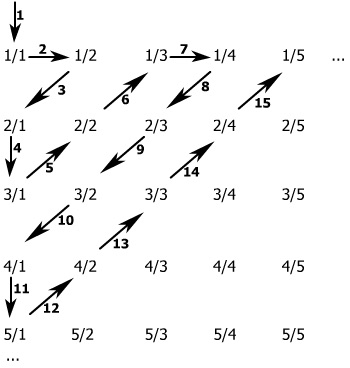
\includegraphics[scale=0.5]{image008.jpg}
\end{center}
\paragraph*{Условие}
в) Множество рациональных чисел сегмента $\left[ a, b\right] $ счетно при a < b
\paragraph*{Доказательство}
Множество рациональных чисел сегмента $\left[ a, b\right] $ - беконечно. (тк множество плотно)\\
$\Rightarrow$ оно не менее чем счетно. Но по доказанному выше оно не более, чем счетно $\Rightarrow$ счетно.
\paragraph*{Условие}
г) Множество пар $ \left\langle  x, y \right\rangle $, где х и у - рациональные числа, счетно
\paragraph*{Доказательство}
Множество рациональных чисел счетно.\\
Тогда выпишем все рациональный числа сеткой и докажем, что кол-во пар сечтно аналогично доказатульству 4.15 б\\

\subsection*{$\S$ 4.16}
\paragraph*{Условие}
Доказать, что множество всех конечных последовательностей, составленных из элементов некотрого счетного множества, есть счетное множество.
\paragraph*{Доказательство}
Докажем, что множество последовательностей длины n счетно.\\
Используя 4.15 Г мы знаем, что $\aleph_0 * \aleph_0 = \aleph_0$\\
$ \Rightarrow $ $\aleph_0^{n} = \aleph_0 $.\\
Кол-во последовательностей конченой длиный счетно $\Rightarrow$ множество всех последедовательностей конечной длинны тоже счетно.


\subsection*{$\S$ 4.18}
\paragraph*{Условие}
Доказать, что множество многочленов от одной переменной с целыми коэффицентами счетно.
\paragraph*{Доказательство}
Многочлен от одной переменно с целыми коэффицентами представляет из себя конечную последовательных целых чисел $\Rightarrow$ сводится к задаче 4.16

\subsection*{$\S$ 4.19}
\paragraph*{Условие}
Доказать счетность множетсва алгебраических чисел, т. е. чисел, являющихся корнями многочленов от одной переменной с целыми коэвицентами.
\paragraph*{Доказательство}
Кол-во корней у многочлена степени n не более, чем n.\\
Тк кол-во многочленов с целыми коеффицентами от одной перменной счетно (по задаче 4.18), то и кол-во корней счетно.\\
Тк можем пронумеровать.

\subsection*{$\S$ 4.20}
\paragraph*{Условие}
Доказать, что любое множество попарно непересекающихся открытых интервалов на действительной прямой не более чем счетно.
\paragraph*{Доказательство}
Кол-во рациональных чисел счетно. А в каждом интервале есть хотя бы одно рациональное число $\Rightarrow$ интервалов не более чем счетное кол-во.

\subsection*{$\S$ 4.23}
\paragraph*{Условие}
Доказать, что множетсво точек разрыва монотонной функции на дейсвтительной оси не более, чем счетно.
\paragraph*{Доказательство}
У монотонной функции каждая точка разрыва соответствует интервалу на оси Y\\
Эти интервалы попарно непересекающиеся $\Rightarrow$ по здадаче 4.20 множесво не более, чем счетно.

\subsection*{$\S$ 4.24}
\paragraph*{Условие}
Доказать, что:\\
a) $\left( 0, 1\right)  \sim \left[  0, 1 \right]  \sim \left(  0, 1 \right]  \sim \left[  0, 1 \right) $\\
\paragraph*{Доказательство}\mbox{}\\
$\left( 0, 1\right)  \sim \left[  0, 1 \right]$\\
$1/2 \leftrightarrow 0$\\
$1/4 \leftrightarrow 1$\\
$1/k^n \leftrightarrow 4/k^n$\\
остальные числа переведем в себя же соответственно\\
$\left(  0, 1 \right]  \sim \left[  0, 1 \right]$\\
$1 \leftrightarrow 1$\\
$1/2 \leftrightarrow 0$\\
$1/k^n \leftrightarrow 2/k^n$\\
остальные числа переведем в себя же соответственно\\
$\left(  0, 1 \right]  \sim \left[  0, 1 \right)$\\
$x \leftrightarrow 1/2 - \mid 1/2 - x \mid$ (симметрично отнасительно 1/2)
\paragraph*{Условие}
б) $\left[ a, b \right]  \sim \left[  c, d \right] $, где $a < b, c < d$\\
\paragraph*{Доказательство}\mbox{}\\
\begin{center}
  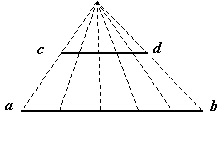
\includegraphics[scale=0.7]{image007.jpg}
\end{center}

\paragraph*{Условие}
в) $\left[ a, b \right] \sim \mathbb{D}$
\paragraph*{Доказательство}\mbox{}\\
по пункту а) $\left( 0, 1\right)  \sim \left[  0, 1 \right]$\\ 
\begin{center}
  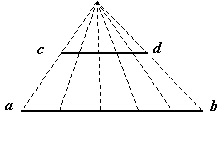
\includegraphics[scale=0.7]{image007.jpg}
\end{center}

\subsection*{$\S$ 4.30}
\paragraph*{Условие}
Какова мощность иррациональных чисел?
\paragraph*{Доказательство}
1)Множество иррациональных чисел более чем счетно.\\
Доказательство.\\
Пусть оно счетно. Выпившем все числа по порядку.\\
\begin{center}
  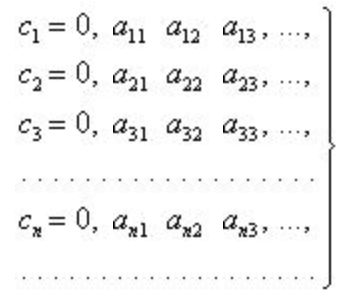
\includegraphics[scale=0.7]{image006.png}
\end{center}
Построим теперь число $C=0, b_1 b_2 b_3 b_4 b_5...$\\
Так что $b_i \neq 0, b_i \neq 9, b_i \neq a_{ii}$\\
Получаем, число, которого нет в таблице, но которое является иррациональным.   


\subsection*{$\S$ 4.31}
\paragraph*{Условие}
Доказать существование трансцендентых (неалгебраических) чисел.
\paragraph*{Доказательство}
Докажем от противного.\\
Пусть их нет. Тогда $ \mathbb{R} \sim $ множество алгебраицеских чисел.\\
Но $ \mathbb{R} $ более чем счетно, а множество всех алгебраических чисел счетно\\
$\Rightarrow$ существуют неалгебраические числа.

\subsection*{$\S$ 4.36}
\paragraph*{Условие}
\paragraph*{Решение}

\subsection*{$\S$ 4.38}
\paragraph*{Условие}
\paragraph*{Решение}

\subsection*{$\S$ 4.39}
\paragraph*{Условие}
\paragraph*{Решение}

\subsection*{$\S$ 4.42}
\paragraph*{Условие}
\paragraph*{Решение}

\section{Отношение эквивелентности}
\subsection*{$\S$ 3.6}
\paragraph*{Условие}
Построить бинарное отношение\\
a)рефлексивное, симметричное, не транзитивное\\
\paragraph*{Решение}
a - нормированное пространство\\
$ r \subseteq a \ast a : (x,y) \in r \leftrightarrow \parallel x - y \parallel \leq \delta $\\
реф. : $\forall x \parallel x - x \parallel = 0 \leq s $\\
симм. : $\parallel x - y \parallel = \parallel y -x  \parallel $\\
Транзитивности нет $\parallel x - y \parallel \leq s $ и $ \parallel y - z  \parallel \leq s \Rightarrow \parallel x - z \parallel \leq s $\\
\paragraph*{Условие}
б)рефлексивное, антисимметричное, не транзитивное\\
\paragraph*{Решение}
$ r \subseteq \mathbb{R} \ast \mathbb{R} : (x,y) \in r \leftrightarrow x \leq y \leq x^2 $\\
реф. : $\forall x (x,x) \in r$\\
антисимметрично: $ x \leq y \leq x^2 $ и $ y \leq x \leq y^2 $ $\Rightarrow x=y$\\
не транз. : $ (2,3) \in r, (3,8) \in r , (2,8) \not\in r$\\
\paragraph*{Условие}
в)рефлексивное, не симметричное, транзитивное\\
\paragraph*{Решение}
$ \leq $ на $ \mathbb{R} $ \\
$ x \leq x$ \\
$ x \leq y, y \leq z \rightarrow x \leq z$\\
$ x \leq y \nrightarrow y \leq x$\\
\paragraph*{Условие}
г)антисимметричное, транзитивное, не рефлексивное\\
\paragraph*{Решение}
$ a \in \mathbb{R} $ \\
$ r \subseteq  \mathbb{R} \times \mathbb{R}$ \\
$ r=\{ (a;a) \} $\\

\subsection*{$\S$ 3.7}
\paragraph*{Условие}
a) Построить бинарное отношение, симметричное, транзитивное, но не рефлексивное.
\paragraph*{Решение}
$r\subseteq \mathbb{R} \times \mathbb{R}$\\
$ a \in \mathbb{R}$\\
$ r =\lbrace ( a; a ) \rbrace $\\
\paragraph*{Условие}
б) Доказать, что если R есть транзитивное и симметричное отношение на множестве A и $\delta_R\cup\rho_R = A$, то R есть эквивалентност на A.
\paragraph*{Решение}
тк $\delta_R\cup\rho_R = A$, то $\exists x \in a \exists y:$\\
либо $(x, y) \in R$ либо $(y, x) \in R$ \\
Из симметричности $(x, y) \in R \wedge (y, x) \in R \rightarrow (x, x) \in R$\\
Те R - отношение эквивалентности.

\subsection*{$\S$ 3.8}
\paragraph*{Условие}
Доказать, что если R симметрично и антисимметрично, то оно транзитивно
\paragraph*{Решение}
Симметричность $(x, y) \in R \rightarrow (y, x) \in R$\\
Антисимметричность $(x, y) \in R \wedge (y, x) \in R \rightarrow y = x$\\
Значит в R лежат только пары вида (x, x) $\Rightarrow$ транзитивно

\subsection*{$\S$ 3.9}
\paragraph*{Условие}
Доказать,что отношение R на множестве a является одновременно эквивалентностью и частичным порядком тогда и только тогда, когда $ R = i_a$
\paragraph*{Решение}
Если $ R = i_a$, то очевидно выоплены рефлексивность, симметричность, антисимметричность и транзитивность.\\
Обратно:\\
Рефлексивность $\Rightarrow \forall x \in a (x, x) \in R \Rightarrow i_a \in R$\\
Сииметричность и антисимметричность $ x = y \Rightarrow R \in  i_a $

\subsection*{$\S$ 3.11}
\paragraph*{Условие}
a - множество всех прямых в $\mathbb{R}^2$, являются ли эквивалентностями следующие отношения?
a) параллельность
б) перпендикулярность
\paragraph*{Решение}
a) является $ a \parallel x $\\
$ x \parallel y \rightarrow y \parallel x$\\
$ x \parallel y \wedge  y \parallel z \rightarrow x \parallel z $\\
б) нет $ \neg x \bot x $ 

\subsection*{$\S$ 3.12}
\paragraph*{Условие}
Определим на $\mathbb{R}$ отношение\\
 a r b $\leftrightarrow$ (a - b) $ \in \mathbb{Q}$\\
Доказать, что r - эквивалентность
\paragraph*{Решение}
a - a = 0 $ \in \mathbb{Q}$\\
a - b $ \in \mathbb{Q} \rightarrow (b - a)=-(a - b) \in \mathbb{Q}$\\
$(a - b) \in \mathbb{Q} (b - c)  \in \mathbb{Q} \rightarrow (a - c) - (a - b) + (b - c) \in \mathbb{Q}$ 

\subsection*{$\S$ 3.17}
\paragraph*{Условие}
Доказать, что сущесвуют взаимоодназначные соотвествия между классом всех разбиений множества а и семествой всех отношений эквивалентности на a
\paragraph*{Доказательство}
Разбиение $\{a_i\}_{i\in\mathbb{I}}$ ставит в соответствие $(x, y) \in r \leftrightarrow \exists i: x \in a_i , y \in a_i$

\subsection*{$\S$ 3.19}
\paragraph*{Условие}
\paragraph*{Решение}

\subsection*{$\S$ 3.20}
\paragraph*{Условие}
Доказать, что пересечение системы эквивалентностей на а есть эквивалентность.
\paragraph*{Решение}
Рассмотрим $\mycap\limits_{i \in X} r_i $\\
$\forall x \in a  \forall i \in X (x,x) \in r_i \rightarrow (x,x) \in \mycap\limits_{i \in X} r_i -$ - рефлексивность\\
$(x,y) \in \mycap\limits_{i \in X} r_i \rightarrow \forall i \in X (x,y) \in r_i \rightarrow \forall i \in X (y,x) \in r_i \rightarrow (y,x) \in \mycap\limits_{i \in X} r_i$ - симметричность\\
\begin{equation*}
\begin{cases} 
(x,y) \in  \mycap\limits_{i \in X} r_i \\
(y,x) \in  \mycap\limits_{i \in X} r_i \\
\end{cases} \rightarrow
\begin{cases} 
\forall i \in X (x,y) \in   r_i \\
\forall i \in X (y,z) \in   r_i \\
\end{cases} 
\rightarrow
\forall i \in X (x,z) \in r_i \rightarrow (x,z) \in \mycap\limits_{i \in X} r_i
\end{equation*}
транзитивность
\section{Упорядоченные множества и ординальные числа}
\subsection*{$\S$ 3.30}
\paragraph*{Условие}
a)Доказать,что всякое частично упорядоченно множество содержит не более одного наибольшего элемента.
б)Доказать, что наибольший (наименьший) элемент частично упорядоченного множества является единственным максимальным(минимальным) элементом.
в)Построить пример частично упорядоченного множества, имеющего точно один минимальный элемент, но не имеющего наименьшего элемента.
\paragraph*{Решение}
а) и б) доказываются от противного.
в) Возьмем множество всех целых чисел, где нет наименьшего и минимального элемента и добавим к этому множеству элемент а, котороый ни с одним из остальных не сравним, что делает его минимальным, но не наименьшим. Получаем множество с 1 минимальным и без наименьших.
\subsection*{$\S$ 3.39}
\paragraph*{Условие}
Доказать, что любое частично упорядоченное множество A изоморфно некоторой системе подмножеств А, упорядечнной вклчением $ \subseteq $.
\paragraph*{Решение}
Докажем по построению. Построим систему подмножеств начиная с минимальных и наименьших элементов. Построим из них множества из 1ого элемента, дальше, возьмем эелемнты которые сравнимы с ними и прибавим к ним эти элементы. И опять найдем наименьшеи и минимальных, убрав предыдущие.

\subsection*{$\S$ 3.42}
\paragraph*{Условие}
Построить линейный порядок на множестве:\\
a) $ \mathscr{N}^2 $\\
б) $ \mathscr{N} \cup \mathscr{N}^2 \cup ... \cup \mathscr{N}^n \cup $\\
в) $ \mathscr{B}$ компелксных чисел
\paragraph*{Решение}\mbox{}\\
а) $ ( m_1, n_1 )  \leq  ( m_2, n_2 )  \Leftrightarrow  (m_1 \leq m_2)  \vee  ( ( m_1 = m_2)  \wedge  ( n_1 \leq n_2 ) ) $ \\
б) $ (m_1, m_2, ..., m_l) \leq (n_1, n_2, ..., n_k) \Leftrightarrow [ \exists i: (i < min(l,k)) | [ (m_1 = n_1) \wedge (m_2 = n_2) \wedge ... \wedge (m_{i-1} = m_{i-1}) \wedge (m_i \leq n_i) ] ] \vee [ (l \leq k) \wedge (m_1 = n_1) \wedge (m_2 = n_2) \wedge ... \wedge (m_{l} = n_{l}) ]$ \\
в) $a + bi \leq c + di \Leftrightarrow [ (a < c) \vee ( (a = c) \wedge (b \leq d) ) ] $\\

\subsection*{$\S$ 3.49}
\paragraph*{Условие}\mbox{}\\
Будем говорить, что частично упорядоченное множество А удовлетворяет \\
(1) условию минимальности, если всякое непустое подмножество M множества А обладает по крайней мере одним минимальным элементом;\\
(2) условию обрыва убывающих цепей, если всякая строго убывающая цепь А конечна;\\
(3) условию индуктивности, если для любого свойства Т выполнено следующее:\\
пусть для любого элемента $a \in A$ из справедливости свойства Т для всех элементов, строго меньших а, вытекает страведливость Т для а; тогда свойством Т обладают все элементы множества А.\\
Доказать эквивалентность всех этих условий.
\paragraph*{Решение}\mbox{}\\
(1) $\Rightarrow$ (2)\\
Возьмем строго убывающую цепь, бесконечную: $x_1 > x_2 > ...$\\
Она не имеет минимального элемента $\Rightarrow$ найдется ее подмножество, у которого не будет минимальных элементов.\\
(2) $\Rightarrow$ (3)\\
Пусть существует свойство Т: для любого элемента $a \in A$ из справедливости свойства Т для всех элементов, строго меньших а, вытекает страведливость Т для а, и пусть существует элемент b, для которого свойство Т не выполняется.\\
Но тогда существует элемент $b_1 < b$ такой, что для него не выполнено свойство T. Тогда для него существует аналогичный элемент $b_2 < b_1$ и т.д.\\
Получили бесконечно строго убывающую цепь.\\
(3) $\Rightarrow$ (1)\\
Пусть есть непустое подмножество M множества А. Пусть есть свойство Т: $ (a \notin A) \vee (\exists$  min  m $\in M )$.\\
Пусть $a in A и \forall b < a $  выполнено Т. Тогда:\\
либо существует элемент c < a, c $\in$ M (для с выполнено Т $\Rightarrow$ в М существует минимальный элемент),  либо такого c не существует (тогда a $\notin$ M или a $\in$ M и а - мниимальный элемент М). Получается, что для а выполнено Т.\\
Пусть теперь M$\neq \varnothing, a \in M$. Тогда M имеет минимальный элемент.

\subsection*{$\S$ 3.54}
\paragraph*{Условие} Доказать, что любое подмножество множества P(A), частично упорядоченное по включению, имеет точную верхнюю грань и точную нижнюю грань.
\paragraph*{Решение}


\subsection*{$\S$ 5.38}
\paragraph*{Условие}
\paragraph*{Решение}

\subsection*{$\S$ 5.46}
\paragraph*{Условие}
\paragraph*{Решение}

\subsection*{$\S$ 5.47}
\paragraph*{Условие}
\paragraph*{Решение}

\subsection*{$\S$ 5.48}
\paragraph*{Условие}
\paragraph*{Решение}

\subsection*{$\S$ 5.50}
\paragraph*{Условие}
\paragraph*{Решение}

\subsection*{$\S$ 5.51}
\paragraph*{Условие}
\paragraph*{Решение}

\end{document}
